\documentclass[11pt]{article}
\usepackage[margin=1in]{geometry}
\usepackage{amssymb,amsfonts,amsmath,amsthm,amscd,dsfont,mathrsfs,bbold}
\usepackage{blkarray}
\usepackage{graphicx,float,psfrag,epsfig,color}
\usepackage{microtype}
\usepackage[pdftex,pagebackref=true,colorlinks]{hyperref}
\usepackage{tikz}
\usepackage{natbib}
\usepackage{listings}

\usepackage{bm}
\usetikzlibrary{positioning}
\tikzset{main node/.style={circle,fill=white!20,draw,minimum size=1cm,inner sep=0pt},}
\hypersetup{linkcolor=[rgb]{.7,0,0}}
\hypersetup{citecolor=[rgb]{0,.7,0}}
\hypersetup{urlcolor=[rgb]{.7,0,.7}}

\newcommand{\remove}[1]{}
\setlength{\topmargin}{0.2in} \setlength{\headheight}{0in}
\setlength{\headsep}{0in} \setlength{\textheight}{8.7in}
\setlength{\topsep}{0in} \setlength{\itemsep}{0in}
\parskip=0.060in

\textwidth=6.6in \oddsidemargin=0truecm \evensidemargin=0truecm



\hbadness=10000 \vbadness=10000

\setlength{\oddsidemargin}{.25in}
\setlength{\evensidemargin}{.25in} \setlength{\textwidth}{6in}
\setlength{\topmargin}{-0.4in} \setlength{\textheight}{8.5in}

\newcommand{\details}[8]{
	\renewcommand{\thepage}{#1-\arabic{page}}
	\noindent
	\begin{center}
		\framebox{
			\vbox{
				\hbox to 5.78in { {\bf  Advanced Methods in Machine Learning}\hfill #2}
				\vspace{4mm}
				\hbox to 5.78in { {\Large \hfill Exercise #1  \hfill} }
				\vspace{2mm}
				\hbox to 5.78in { {{\it #3} \hfil {\it #4} \hfil {\it #5}} }
				\vspace{2mm}
				\hbox to 5.78in { {{\it #6} \hfil {\it #7} \hfil {\it #8}} }
			}
		}
	\end{center}
	\vspace*{4mm}
}

\newcommand{\lecture}[8]{\details{#1}{#2}{#3}{#4}{#5}{#6}{#7}{#8}}
\DeclareMathOperator*{\argmax}{arg\,max}
\graphicspath{{1c/},{1e/},{1d/}}



\begin{document}
	\lecture{4}{30.5.2018}{Nir Raviv 200683548}{Roi Tabach 203022983}{Andrey Leshenko 322026527}{nirraviv@mail.tau.ac.il}{roi.tabach@gmail.com}{andrey.leshenko@gmail.com}
	
\part*{Q1}

The code implementing VAE is on NOVA at
 \url{~leshchenko/arazim/advanced_ml/public/}.
To run it, you must first \textbf{enable a local Python environment}, by running:
\begin{lstlisting}[language=bash]
$ source ./keras_env/bin/activate.csh
\end{lstlisting}
Now if you run a script using ``python something.py'', this environment will be used.
You can run the trained network in the \url{hw4_trained} folder in the same directory, or first train and then run in \url{hw4_untrained}. If you start a long running task on NOVA, it will usually be killed by the server after a few minutes.
For this reason, if you want to train through an SSH connection to NOVA, first SSH to one of the Shreiber PCs (for example gauss-11) and train there.

\textbf{Important note about plots}:
by default the code will display the plots in a window.
If when connecting to NOVA you passed the -X argument to SSH, you should be able to see these windows.
If opening windows is not possible and you would prefer to save the plots as image files, open the Python code and change \textbf{SAVE\_PLOTS} to True.

The following sections, c,d,e, will be answered for all models: VAE, fixed-variance VAE, and Convolutional VAE. The answers for f,g are going to be included in c-e.

\section*{c}
First we will show the latent-space coordinates of the entire MNIST-dataset, for each of the representations. 

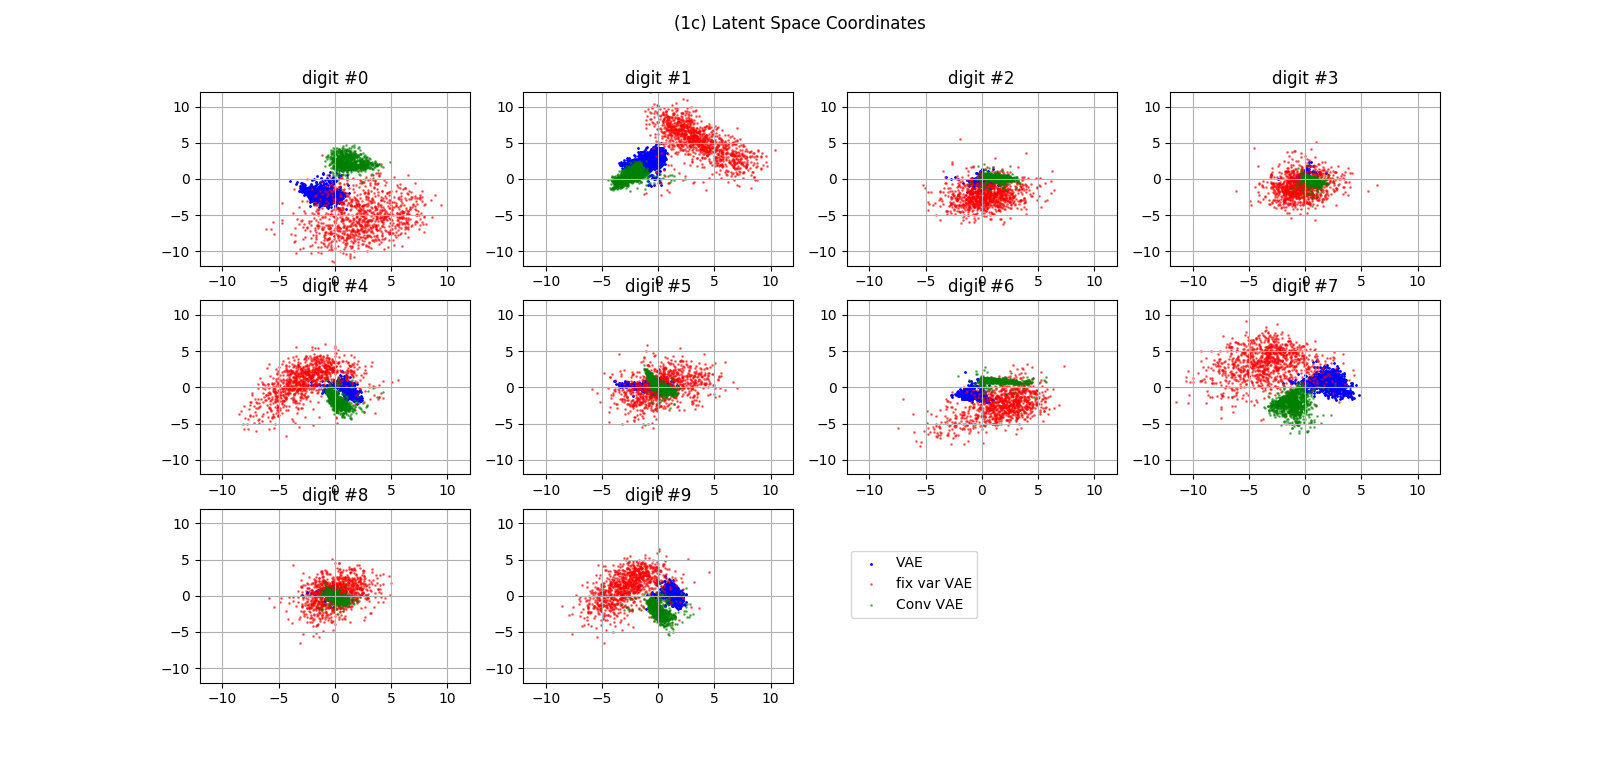
\includegraphics[scale=0.4]{entire_space_coordinates}

As one can see the VAE and Convolutional VAE latent space points have small overlap since their variance is smaller. Therefore, these auto encoders are better. \\
Next we show an example for each of the digits, 0-9 (each in it's seperate row), the representation reconstructed with each of the decoders: left is the VAE, middle is the fixed variance VAE, and right is convolutional VAE.

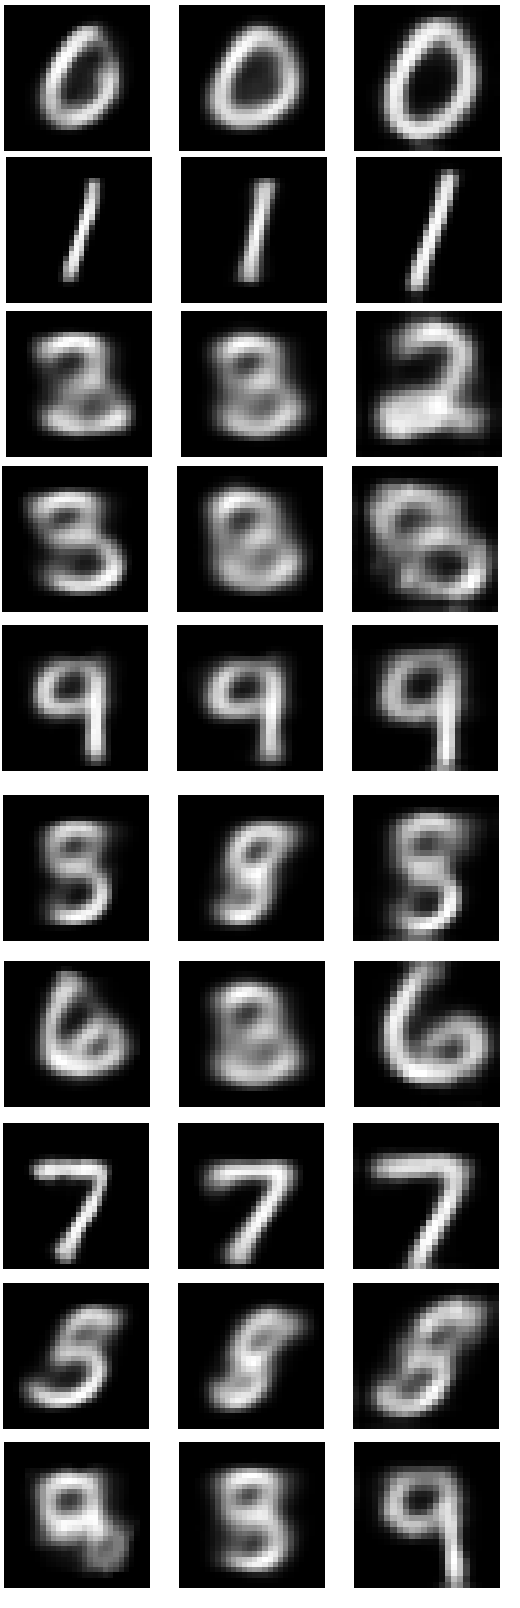
\includegraphics[scale=0.2]{table}

\section*{d}
Here we take decode the latent-space vector $(0.5, 0.2)$ using each of our decoders:
left is the VAE, middle is the fix-var VAE, and rightmost is the conv-VAE.

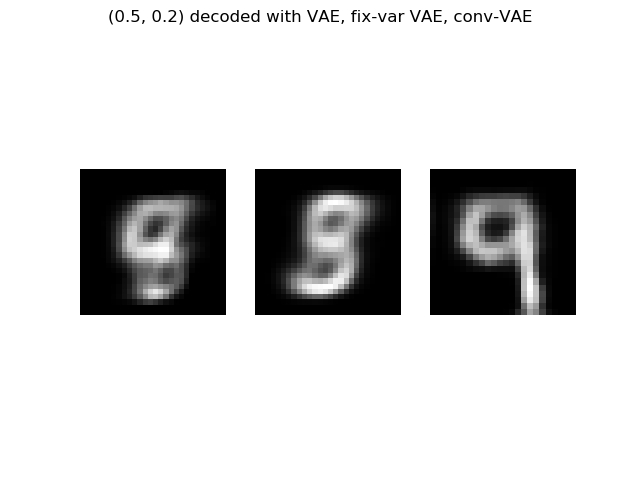
\includegraphics[scale=0.75]{1d}


\section*{e}
Here we show how interpolation between two latent-space points look in the decoded space, using each of our decoders:
VAE:

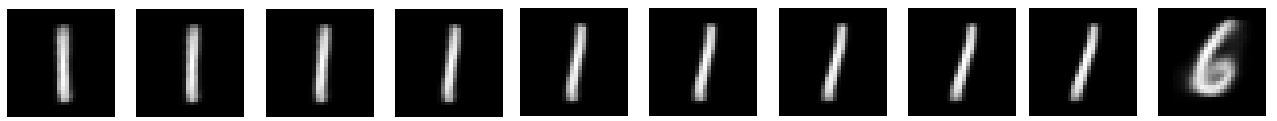
\includegraphics[scale=0.3]{vae}

Fixed Variance:

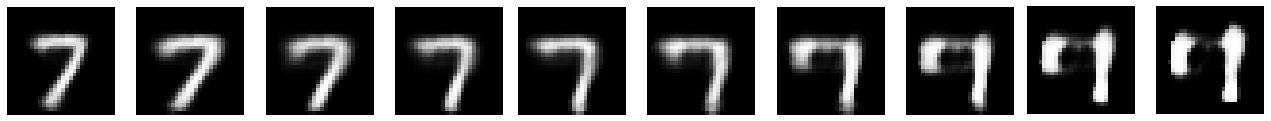
\includegraphics[scale=0.3]{fix}

Convolutional:

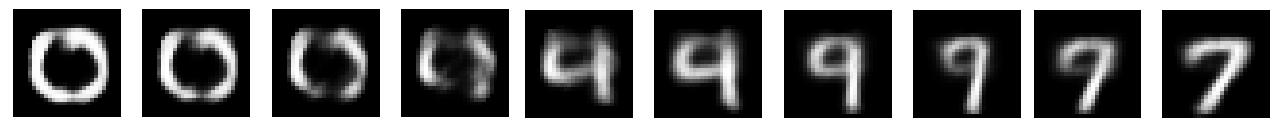
\includegraphics[scale=0.3]{conv}


\part*{Q2}
Given $P \sim \mathcal{N}(\mu_1, \sigma_1^2)$ and $Q \sim \mathcal{N}(\mu_2, \sigma_2^2)$ random variables, we need to derive an expression for the KL divergence of $P$ and $Q$.
\begin{align*}
	\begin{split}
		D_{KL}(P||Q) = \int_{\mathds{R}} p(x) log \left(\frac{p(x)}{q(x)} \right)dx =  \mathds{E}_p[log(p(x))] - \mathds{E}_p[log(q(x))]
	\end{split}\\
	\begin{split}
		\mathds{E}_p[log(p(x))] = \mathds{E}_p\left[log\left(\frac{1}{\sqrt{2\pi\sigma_1^2}}e^{-\frac{(x-\mu_1)^2}{2\sigma_1^2}}\right)\right] =
		-\frac{1}{2}log(2\pi\sigma_1^2) - \frac{1}{2\sigma_1^2}\mathds{E}_p[(x-\mu_1)^2] = \\ -\frac{1}{2}log(2\pi\sigma_1^2) - \frac{1}{2\sigma_1^2}\mathds{E}_p[x^2 - 2x\mu_1 + \mu_1^2] =
		 -\frac{1}{2}log(2\pi\sigma_1^2) - \frac{\sigma_1^2}{2\sigma_1^2} = -\frac{1}{2}log(2\pi\sigma_1^2) - \frac{1}{2}
	\end{split}	\\
	\begin{split}
		\mathds{E}_p[log(q(x))] = \mathds{E}_p\left[log\left(\frac{1}{\sqrt{2\pi\sigma_2^2}}e^{-\frac{(x-\mu_2)^2}{2\sigma_2^2}}\right)\right] = 
		-\frac{1}{2}log(2\pi\sigma_2^2) - \frac{1}{2\sigma_2^2}\mathds{E}_p[(x-\mu_2)^2] = \\
		-\frac{1}{2}log(2\pi\sigma_2^2) - \frac{1}{2\sigma_2^2}\mathds{E}_p[x^2 - 2x\mu_2 + \mu_2^2] = 
		-\frac{1}{2}log(2\pi\sigma_2^2) - \frac{\sigma_1^2+\mu_1^2-2\mu_1\mu_2+\mu_2^2}{2\sigma_2^2} = \\
		-\frac{1}{2}log(2\pi\sigma_2^2) - \frac{\sigma_1^2+(\mu_1-\mu_2)^2}{2\sigma_2^2}
	\end{split}
\end{align*}
Thus,
\begin{equation*}
	D_{KL}(P||Q) = -\frac{1}{2}log(2\pi\sigma_1^2) - \frac{1}{2} + \frac{1}{2}log(2\pi\sigma_2^2) + \frac{\sigma_1^2+(\mu_1-\mu_2)^2}{2\sigma_2^2} = log\left(\frac{\sigma_2}{\sigma_1}\right) - \frac{1}{2} + \frac{\sigma_1^2+(\mu_1-\mu_2)^2}{2\sigma_2^2}
\end{equation*}

\end{document}
